\documentclass[a4paper, dvipsnames]{article}

\usepackage[T1]{fontenc}
\usepackage{geometry}
\geometry{
  left=2cm,
  right=2cm,
  top=4cm,
  bottom=4cm,
  bindingoffset=5mm
}

\usepackage{amssymb} 
\usepackage{amsmath}
\usepackage{amsthm}
\usepackage[utf8]{inputenc}
\usepackage[T1]{fontenc}
\usepackage{lmodern}
\usepackage{ngerman}
\usepackage{scrlayer-scrpage}
\usepackage{ulem}
\usepackage{xcolor}
\usepackage{graphicx}
\usepackage{listings}

\lstset{
language=Java,
aboveskip=3mm,
belowskip=3mm,
showstringspaces=false,
keywordstyle=\color{OliveGreen},
commentstyle=\color{gray},
breaklines=true,
breakatwhitespace=true,
tabsize=4
}

\pagestyle{scrheadings}

\ihead{Gruppe 10}
\chead{Logische Programmierung}
\ohead{\pagemark}

\setlength{\parindent}{0pt}


\begin{document}

{ \hspace{7,7cm}{\bfseries{Serie 1}}  {\hspace{6,0cm}{Gruppe 10}}\\

Adnan Alyousfi, 218205332, Informatik\\
Dirk Peglow, Informatik\\
Nils Henrik Seitz, 218205308, Informatik\\
Lorka Trad, Informatik\\
Nico Trebbin, 218204402, Informatik\\

\uline{\bfseries{Aufgabe 1}}\\

{\bfseries 1.A}\\

unify({\color{red}f}(g(2, 3), Y ), {\color{red}f}(X, f(2)))\quad$\theta = \{\}$\\
unify(f({\color{red}g(2, 3)}, Y ), f({\color{red}X}, f(2)))\quad$\theta = \{X = g(2,3)\}$\\
unify(f(g(2, 3), {\color{red}Y} ), f(g(2, 3), {\color{red}f(2)}))\quad$\theta = \{X = g(2,3), Y = f(2)\}$\\
unify(f(g(2, 3), f(2) ), f(g(2, 3), f(2)))\quad$\theta = \{X = g(2,3), Y = f(2)\}$\\
$\theta = \{X = g(2,3), Y = f(2)\}$ (Allgemeinster Unifikator)\\

{\bfseries 1.B}\\

unify\{{\color{red}g}(X), {\color{red}f}(X)\}\quad$\theta = \{\}$ - Nicht unifizierbar, da die Funktoren unterschiedlich sind.\\

{\bfseries 1.C}\\

unify({\color{red}f}(X, g(Y, Y )), {\color{red}f}(g(Y, Y ),X))\quad$\theta = \{\}$\\
unify(f({\color{red}X}, g(Y, Y )), f({\color{red}g(Y, Y )},X))\quad$\theta = \{X = g(Y,Y)\}$\\
unify(f(g(Y,Y), \color{red}g(Y, Y )}), f(g(Y, Y ),{\color{red}g(Y,Y)})\quad$\theta = \{X = g(Y,Y)\}$\\
unify(f(g(Y,Y), g(Y, Y )), f(g(Y, Y ),g(Y,Y))\quad$\theta = \{X = g(Y,Y)\}$\\
$\theta = \{X = g(Y,Y)\}$ (Allgemeinster Unifikator)\\

{\bfseries 1.D}\\

unify({\color{red}f}(X, g(Y, Y )), {\color{red}f}(g(Y, Y ), Y ))\quad$\theta = \{\}$\\
unify(f({\color{red}X}, g(Y, Y )), f({\color{red}g(Y, Y )}, Y ))\quad$\theta = \{X = g(Y, Y)\}$\\
unify(f(g(Y, Y), g(Y, Y )), f(g(Y, Y ), Y ))\quad$\theta = \{X = g(Y, Y)\}$\\ - Nicht unifizierbar, da Y im Term g(Y, Y) auftaucht. Beim unifizieren würde dies zu einer Endlosschleife führen.\\


\uline{\bfseries{Aufgabe 2}}\\
{\bfseries 2.B}\\
\center{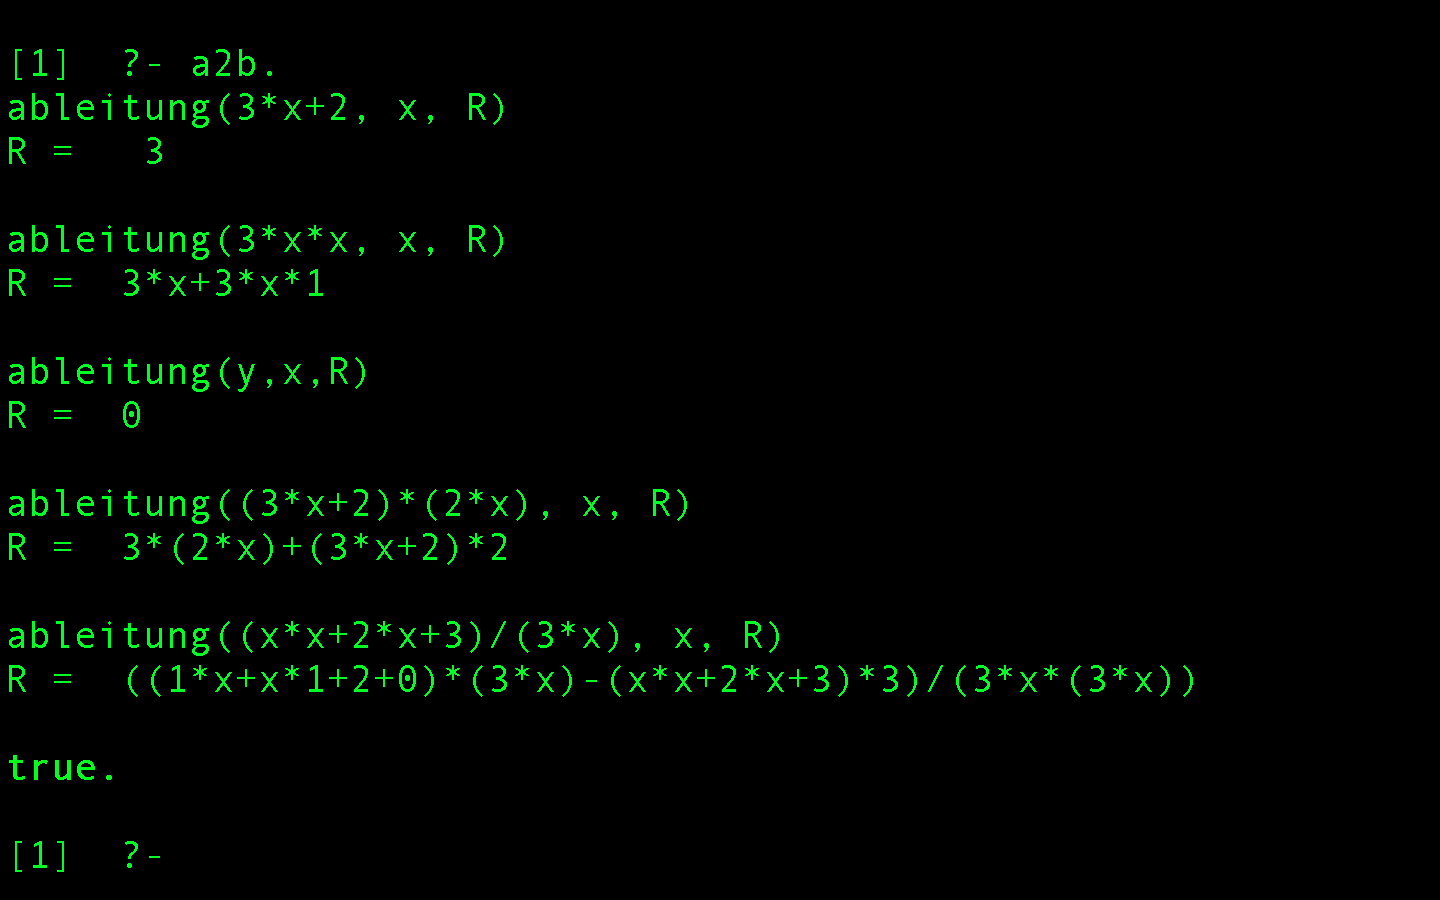
\includegraphics[width=0.6\textwidth]{Data/A2/1.png}} \\
\end{document}